\documentclass[style=sailor,size=12pt]{powerdot}
\usepackage{epic,array,ecltree,url,calrsfs}
\usepackage[nointegrals]{wasysym}
\usepackage{listings}
\usepackage{epsfig}
\usepackage{amsmath}
\usepackage{amsfonts}
\usepackage{amssymb}
\usepackage{amsxtra}
\usepackage{amsthm}
\usepackage{mlextra} % Must be below ams packages
\usepackage{mathrsfs}
\usepackage{color}
\usepackage{array}
\usepackage{graphicx}
\graphicspath{ {../art/} }
\usepackage{bm}
\usepackage{tikz}
\usepackage{multicol}
\usepackage{enumitem}

\pdsetup{method=normal}
\begin{document}

\begin{wideslide}[bm=,toc=]{On-off switch}
\begin{program}
while (true) \{ \\
\hspace{1em}push() \\
\hspace{1em}$\dots$ \\
\hspace{1em}push() \\
\}
\end{program}
\begin{figure}[h]
\centering
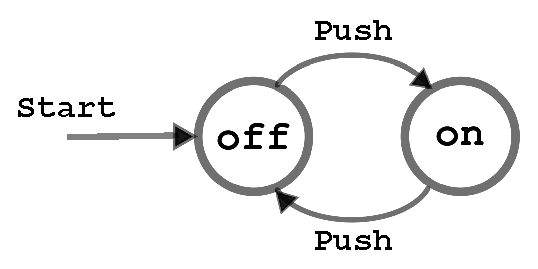
\includegraphics[width=2.5in, height=.75in,keepaspectratio=true]{switch.eps}
\caption{A finite automaton modeling an on/off switch}
\label{2sp}
\end{figure}
\end{wideslide}

\begin{wideslide}[bm=,toc=]{Peterson's algorithm}
\begin{center}
\begin{tabular}{|p{0.46\textwidth}|p{0.46\textwidth}|}
\hline
\multicolumn{2}{|c|}{\p{boolean wantp = false, wantq = false}}\\
\multicolumn{2}{|c|}{\p{int turn = 1}}\\\hline
\p{Process p} & \p{Process q} \\
\hline
\p{while (true) \{} & \p{while (true) \{} \\
\p{\ \ non-critical-section} & \p{\ \ non-critical-section} \\
\p{\ \ wantp = true} & \p{\ \ wantq = true} \\
\p{\ \ turn = 1} & \p{\ \ turn = 2} \\
\p{\ \ wait until } & \p{\ \ wait until } \\
\p{\ \ \ \ (!wantq or turn == 2)} & \p{\ \ \ \ (!wantp or turn == 1)} \\
\p{\ \ critical-section} & \p{\ \ critical-section} \\
\p{\ \ wantp = false} & \p{\ \ wantq = false} \\
\p{\}} & \p{\}} \\\hline
\end{tabular}
\end{center}
\end{wideslide}

\begin{wideslide}[bm=,toc=]{Abbreviated algorithm}
\begin{center}
\begin{tabular}{|p{0.46\textwidth}|p{0.46\textwidth}|}
\hline
\multicolumn{2}{|c|}{\p{boolean wantp = false, wantq = false}}\\
\multicolumn{2}{|c|}{\p{int turn = 1}}\\\hline
\p{Process p} & \p{Process q} \\
\hline
\p{while (true) \{} & \p{while (true) \{} \\
\p{\ tryp: wantp=true; turn=1} & \p{\ tryq: wantq=true; turn=2} \\
\p{\ waitp: wait until } & \p{\ waitq: wait until } \\
\p{\ \ \ \ \ (!wantq or turn == 2)} & \p{\ \ \ \ \ (!wantp or turn == 1)} \\
\p{\ csp: wantp = false} & \p{\ csq: wantq = false} \\
\p{\}} & \p{\}} \\\hline
\end{tabular}
\end{center}
\end{wideslide}

\begin{wideslide}[bm=,toc=]{Figure 16.3: Finite automata for Peterson's algorithm}
\begin{center}
\unitlength=1.1pt
\begin{picture}(230,180)
%\put(0,0){\framebox(230,180){}}
%process p
\put(0,140){
\put(0,0){
  \put(-20,15){\vector(1,0){18}}
  \put(15,15){\circle{30}}
  \put( 0, 0){\makebox(30,30){\p{tryp}}}
  \put(32,15){\vector(1,0){66}}
  \put(30,17){
     \makebox(70,20){\shortstack[l]{\p{wantp=true}\\\p{turn=1}}}
  }
}
\put(100,0){
  \put(15,15){\circle{30}}
  \put( 0, 0){\makebox(30,30){\p{waitp}}}
  \put(32,15){\vector(1,0){66}}
  \put(30,17){
     \makebox(70,20){\shortstack[l]{\p{!wantq or}\\\p{turn == 2}}}
  }
  \put(28,-5){\oval(26,20)[r]}
  \put(2,-5){\oval(26,20)[l]}
  \put(28,-15){\line(-1,0){26}}
  \put(-3,5){\vector(1,0){5}}
  \put(30,-17){
     \makebox(70,20){\shortstack[l]{\p{wantq and}\\\p{turn == 1}}}
  }
}
\put(200,0){
  \put(15,15){\circle{30}}
  \put( 0, 0){\makebox(30,30){\p{csp}}}
  \put(15,-2){\line(0,-1){38}}
  \put(15,-40){\line(-1,0){200}}
  \put(-185,-40){\vector(0,1){38}}
  \put(-120,-43){
     \makebox(70,20){\p{wantp=false}}
  }
}
}

% process q
\put(0,40){
\put(0,0){
  \put(-20,15){\vector(1,0){18}}
  \put(15,15){\circle{30}}
  \put( 0, 0){\makebox(30,30){\p{tryq}}}
  \put(30,15){\vector(1,0){67}}
  \put(30,17){
     \makebox(70,20){\shortstack[l]{\p{wantq=true}\\\p{turn=2}}}
  }
}
\put(100,0){
  \put(15,15){\circle{30}}
  \put( 0, 0){\makebox(30,30){\p{waitq}}}
  \put(30,15){\vector(1,0){67}}
  \put(30,17){
     \makebox(70,20){\shortstack[l]{\p{!wantp or}\\\p{turn == 1}}}
  }
  \put(28,-5){\oval(26,20)[r]}
  \put(2,-5){\oval(26,20)[l]}
  \put(28,-15){\line(-1,0){26}}
  \put(-3,5){\vector(1,0){5}}
  \put(30,-17){
     \makebox(70,20){\shortstack[l]{\p{wantp and}\\\p{turn == 2}}}
  }
}
\put(200,0){
  \put(15,15){\circle{30}}
  \put( 0, 0){\makebox(30,30){\p{csq}}}
  \put(15,0){\line(0,-1){40}}
  \put(15,-40){\line(-1,0){200}}
  \put(-185,-40){\vector(0,1){40}}
  \put(-120,-43){
     \makebox(70,20){\p{wantq=false}}
  }
}
}
\end{picture}
\end{center}
\end{wideslide}

\end{document}
